\section{构建阀三维模型}
\subsection{构建B-B段实体}
\begin{procedure}
\item 建立图层。

建立“中心线”和“实线”两个图层,并将当前图层设置为“中心线”图层。
\item 切换视图方向为左视图。
\item 绘制中心线,其结果如图\ref{fig:fabancenterline}所示。

绘制$B-B$段对称中心线。
\begin{lstlisting}
|命令: XLINE|
|指定点或 [水平(H)/垂直(V)/角度(A)/二等分(B)/偏移(O)]:|
|指定通过点:$ @1<0$|
|指定通过点:$ @1<90$|
|指定通过点:|
\end{lstlisting}
绘制$M4$螺孔中心线。
\begin{lstlisting}
|命令: C CIRCLE|
|指定圆的圆心或 [三点(3P)/两点(2P)/切点、切点、半径(T)]:|
|指定圆的半径或 [直径(D)]: 19.5|
\end{lstlisting}
\begin{figure}[htbp]
\centering
\begin{floatrow}[3]
\ffigbox{\caption{绘制中心线}\label{fig:fabancenterline}}{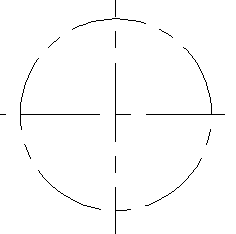
\includegraphics[scale=0.5]{fabancenterline.png}}
\ffigbox{\caption{偏移}\label{fig:fabana-a1}}{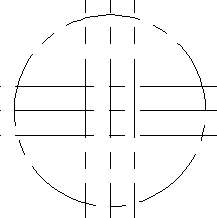
\includegraphics[scale=0.5]{fabana-a1.png}}
\ffigbox{\caption{绘制$\phi 42$圆}\label{fig:fabana-a2}}{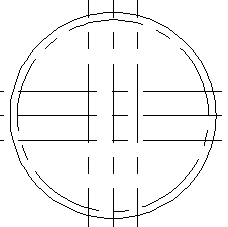
\includegraphics[scale=0.5]{fabana-a2.png}}
\end{floatrow}
\end{figure}
\item 绘制十字体。

偏移产生十字线,结果如图\ref{fig:fabana-a1}所示
\begin{lstlisting}
|命令: OFFSET|
|当前设置: 删除源=否  图层=源  OFFSETGAPTYPE=0|
|指定偏移距离或 [通过(T)/删除(E)/图层(L)] $<$通过$>$:  5|
|选择要偏移的对象,或 [退出(E)/放弃(U)] $<$退出$>$:|
|指定要偏移的那一侧上的点,或 [退出(E)/多个(M)/放弃(U)]$<$退出$>$:|
|选择要偏移的对象,或 [退出(E)/放弃(U)] $<$退出$>$:|
|指定要偏移的那一侧上的点,或 [退出(E)/多个(M)/放弃(U)]$<$退出$>$:|
|选择要偏移的对象,或 [退出(E)/放弃(U)]$<$退出$>$:|
|指定要偏移的那一侧上的点,或 [退出(E)/多个(M)/放弃(U)]$<$退出$>$:|
|选择要偏移的对象,或 [退出(E)/放弃(U)]$<$退出$>$:|
|指定要偏移的那一侧上的点,或 [退出(E)/多个(M)/放弃(U)]$<$退出$>$:|
|选择要偏移的对象,或 [退出(E)/放弃(U)] $<$退出$>$:|
\end{lstlisting}
绘制$\phi 42$圆,结果如图\ref{fig:fabana-a2}所示。
\begin{lstlisting}
|命令: CIRCLE|
|指定圆的圆心或 [三点(3P)/两点(2P)/切点、切点、半径(T)]:|
|指定圆的半径或 [直径(D)] <19.5000>: 21|
\end{lstlisting}
修剪完成十字形(命令提示省略),结果如图\ref{fig:fabana-a3}所示。
\begin{figure}[htbp]
\centering
\begin{floatrow}[3]
\ffigbox{\caption{修剪结果}\label{fig:fabana-a3}}{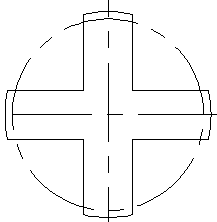
\includegraphics[scale=0.5]{fabana-a3.png}}
\ffigbox{\caption{拉伸}\label{fig:fabana-a4}}{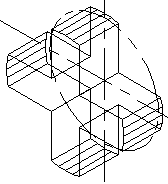
\includegraphics[scale=0.5]{fabana-a4.png}}
\ffigbox{\caption{绘制$\phi 50$圆柱}\label{fig:fabana-a5}}{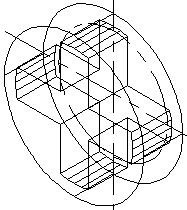
\includegraphics[scale=0.5]{fabana-a5.png}}
\end{floatrow}
\end{figure}

面域十字形。
\begin{lstlisting}
|命令: REG REGION|
|选择对象: 找到 12 个|
|选择对象:|
\end{lstlisting}
切换视图方向为西南等轴测,拉伸构建十字体,其结果如图\ref{fig:fabana-a4}所示。
\begin{lstlisting}
|命令: EXTRUDE|
|当前线框密度:  ISOLINES=4,闭合轮廓创建模式 = 实体|
|选择要拉伸的对象或 [模式(MO)]: 找到 1 个|
|选择要拉伸的对象或 [模式(MO)]:|
|指定拉伸的高度或 [方向(D)/路径(P)/倾斜角(T)/表达式(E)]: -14|
\end{lstlisting}
\item 绘制$\phi 50$圆柱体,其结果如图\ref{fig:fabana-a5}所示。
\begin{lstlisting}
|命令:  CYLINDER|
|指定底面的中心点或 [三点(3P)/两点(2P)/切点、切点、半径(T)|
|/椭圆(E)]:int 于|
|指定底面半径或 [直径(D)]: 25|
|指定高度或 [两点(2P)/轴端点(A)]: -14|
\end{lstlisting}
\newpage
\item 绘制$\phi 42$圆柱体。
\begin{lstlisting}
|命令:  CYLINDER|
|指定底面的中心点或 [三点(3P)/两点(2P)/切点、切点、半径(T)|
|/椭圆(E)]:int 于|
|指定底面半径或 [直径(D)]$<$25.0000$>$: 21|
|指定高度或 [两点(2P)/轴端点(A)]$<$-14.0000$>$: |
\end{lstlisting}
\begin{figure}[htbp]
\centering
\begin{floatrow}[3]
\ffigbox{\caption{绘制$\phi 32$圆柱}\label{fig:fabana-a6}}{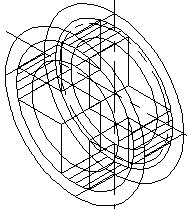
\includegraphics[scale=0.8]{fabana-a6.png}}
\ffigbox{\caption{差集结果}\label{fig:fabana-a7}}{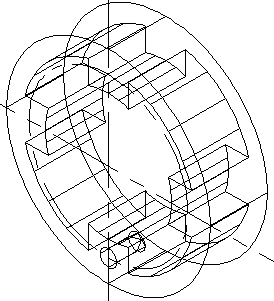
\includegraphics[scale=0.5]{fabana-a7.png}}
\ffigbox{\caption{生成螺孔结果}\label{fig:fabana-a8}}{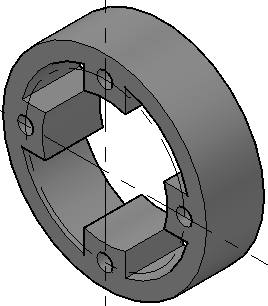
\includegraphics[scale=0.5]{fabana-a8.png}}
\end{floatrow}
\end{figure}
\item 绘制$\phi 31$圆柱体,结果如图\ref{fig:fabana-a6}所示。
\begin{lstlisting}
|命令:  CYLINDER|
|指定底面的中心点或 [三点(3P)/两点(2P)/切点、切点、半径(T)|
|/椭圆(E)]:int 于|
|指定底面半径或 [直径(D)]$<$21.0000$>$: 15.5|
|指定高度或 [两点(2P)/轴端点(A)]$<$-14.0000$>$: |
\end{lstlisting}
\item 合成$B-B$段实体。

从$\phi 50$圆柱体中减去$\phi 42$圆柱体。
\begin{lstlisting}
|命令: SUBTRACT|
|选择要从中减去的实体、曲面和面域...|
|选择对象: 找到 1 个|
|选择对象:  选择要减去的实体、曲面和面域...|
|选择对象: 找到 1 个|
|选择对象:|
\end{lstlisting}
并入十字体。
\begin{lstlisting}
|命令: UNION|
|选择对象: 找到 1 个|
|选择对象: 找到 1 个,总计 2 个|
|选择对象:|
\end{lstlisting}
减去$\phi 31$圆柱体,结果如图\ref{fig:fabana-a7}所示。
\begin{lstlisting}
|命令: SUBTRACT|
|选择要从中减去的实体、曲面和面域...|
|选择对象: 找到 1 个|
|选择对象:  选择要减去的实体、曲面和面域...|
|选择对象: 找到 1 个|
|选择对象:|
\end{lstlisting}
\item 绘制$M4$螺孔圆柱体。
\begin{lstlisting}
|命令:  CYLINDER|
|指定底面的中心点或 [三点(3P)/两点(2P)/切点、切点、半径(T)|
|/椭圆(E)]:int 于|
|指定底面半径或 [直径(D)]$<$15.5000$>$: 2|
|指定高度或 [两点(2P)/轴端点(A)]$<$-14.0000$>$:-7 |
\end{lstlisting}
\item 绘制$M4$螺孔退刀圆锥。

启动绘制圆锥体命令的方法有:
\begin{itemize}
\item 键盘输入CONE\index{cone}。
\item 【绘图】$\rightarrow$【建模】$\rightarrow$【圆锥体】。
\item 【建模】$\triangleright$【圆锥体】图标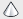
\includegraphics[scale=0.6]{cone.png}。
\end{itemize}
\begin{lstlisting}
|命令: cone|
|指定底面的中心点或 [三点(3P)/两点(2P)/切点、切点、半径(T)|
|/椭圆(E)]:|
|指定底面半径或 [直径(D)] $<$2.0000$>$:|
|指定高度或 [两点(2P)/轴端点(A)/顶面半径(T)] $<$-7.0000$>$: -1|
\end{lstlisting}
\begin{lstlisting}
|命令: UNION|
|选择对象: 找到 1 个|
|选择对象: 找到 1 个,总计 2 个|
|选择对象:|
\end{lstlisting}
\item 阵列生成4个$M4$螺孔圆柱。
\begin{lstlisting}
|命令: 3darray|
|选择对象: 找到 1 个|
|选择对象:|
|输入阵列类型 [矩形(R)/环形(P)]$<$矩形$>$:p|
|输入阵列中的项目数目: 4|
|指定要填充的角度 (+=逆时针, -=顺时针)$ <360>$:|
|旋转阵列对象? [是(Y)/否(N)] $<Y>$:|
|指定阵列的中心点:|
|指定旋转轴上的第二点:|
\end{lstlisting}
\newpage
用差集生成最螺孔,其结果如图\ref{fig:fabana-a8}
\begin{lstlisting}
|命令: SUBTRACT|
|选择要从中减去的实体、曲面和面域...|
|选择对象: 找到 1 个|
|选择对象:  选择要减去的实体、曲面和面域...|
|选择对象: 指定对角点: 找到 4 个|
|选择对象:|
\end{lstlisting}
\item 生成$R3$空间圆弧,结果如图\ref{fig:fabana-a9}所示。
\begin{lstlisting}
|命令:  FILLETEDGE|
|半径 = 1.0000|
|选择边或 [链(C)/环(L)/半径(R)]: r|
|输入圆角半径或 [表达式(E)] <1.0000>: 3|
|选择边或 [链(C)/环(L)/半径(R)]:|
|选择边或 [链(C)/环(L)/半径(R)]:|
|选择边或 [链(C)/环(L)/半径(R)]:|
|选择边或 [链(C)/环(L)/半径(R)]:|
|选择边或 [链(C)/环(L)/半径(R)]:|
|选择边或 [链(C)/环(L)/半径(R)]:|
|选择边或 [链(C)/环(L)/半径(R)]:|
|选择边或 [链(C)/环(L)/半径(R)]:|
|选择边或 [链(C)/环(L)/半径(R)]:|
|已选定 8 个边用于圆角。|
|按 Enter 键接受圆角或 [半径(R)]:|
\end{lstlisting}
\begin{figure}[htbp]
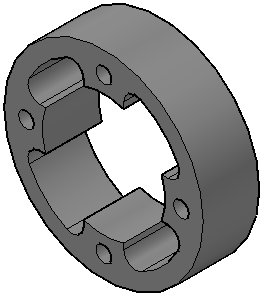
\includegraphics[scale=1]{fabana-a9.png}
\caption{$B-B$段实体结果}\label{fig:fabana-a9}
\end{figure}
\end{procedure}
\endinput
